\documentclass[tikz]{standalone}
\usepackage{tikz}

\begin{document}    
	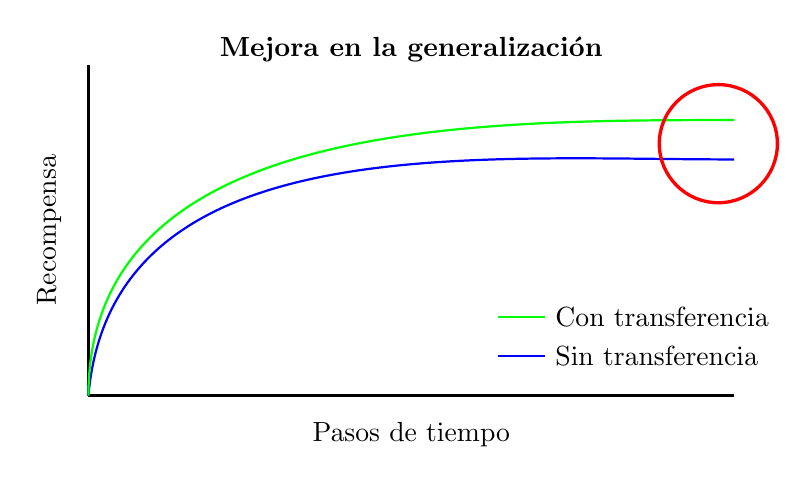
\begin{tikzpicture}
		% Ejes
		\draw[-, very thick] (0, 0) -- (8.2, 0) node [pos=0.5, yshift=-0.5cm] {Pasos de tiempo};
		\draw[-, very thick] (0, 0) -- (0, 4.2) node [pos=0.5, xshift=-0.5cm,rotate=90]{Recompensa};
		
		% Titulo
		\node[font=\bfseries] at (4.1, 4.4) {Mejora en la generalización};	
		
		% Label
		\draw[blue, thick]  (5.2,0.5) -- ++(0.6,0) node[right, text=black] {Sin transferencia};
		\draw[green, thick] (5.2,1.0) -- ++(0.6,0) node[right, text=black] {Con transferencia};
		
		% Lineas
		\draw[blue, thick] (0,0.0) to[out=85, in=180] (8.2,3.0);
		\draw[green, thick] (0,0.0) to[out=90, in=180] (8.2,3.5);  
		
		% Circulo
		\node[circle,draw=red, minimum size=1.5cm,  very thick] (c) at (8.0,3.2) {};
		
			
	\end{tikzpicture}
\end{document}